\documentclass[12pt,a4paper,oneside]{report}

% =============================================================
%  PACKAGES
% =============================================================
\usepackage[utf8]{inputenc}
\usepackage[T1]{fontenc}
\usepackage{mathptmx}                       % Times New Roman (text + math)
\usepackage[top=2.54cm, bottom=2.54cm, left=2.54cm, right=2.54cm]{geometry}
\usepackage{setspace}
\usepackage{graphicx}
\usepackage{amsmath,amssymb,amsfonts}
\usepackage{array}
\usepackage{booktabs}
\usepackage{tabularx}
\usepackage{caption}
\usepackage{subcaption}
\usepackage{enumitem}
\usepackage{fancyhdr}
\usepackage{titlesec}
\usepackage{appendix}
\usepackage{listings}
\usepackage{xcolor}
\usepackage{float}
\usepackage{tocbibind}
\usepackage{microtype}
\usepackage[hidelinks]{hyperref}
\usepackage{natbib}
\usepackage{tikz}
\usetikzlibrary{shapes.geometric, arrows.meta, positioning, fit, backgrounds}
\usepackage{tcolorbox}
\tcbuselibrary{skins}

% =============================================================
%  GLOBAL SETTINGS
% =============================================================
\onehalfspacing
\setlength{\parindent}{1.5em}
\setlength{\parskip}{0.3em plus 0.1em minus 0.1em}
\sloppy

\hypersetup{
    colorlinks=true,
    linkcolor=black,
    citecolor=black,
    urlcolor=blue,
    pdftitle={A Comparative Study of Graph-Based RAG Frameworks},
    pdfauthor={Student Name},
}

% =============================================================
%  CHAPTER / SECTION FORMATTING
% =============================================================
\titleformat{\chapter}[hang]
    {\normalfont\huge\bfseries}{\thechapter}{0.6em}{}
\titlespacing*{\chapter}{0pt}{-10pt}{28pt}

\titleformat{\section}{\normalfont\fontsize{14}{16}\bfseries}{\thesection}{0.75em}{}
\titlespacing*{\section}{0pt}{16pt}{8pt}

\titleformat{\subsection}{\normalfont\fontsize{12}{14}\bfseries}{\thesubsection}{0.75em}{}
\titlespacing*{\subsection}{0pt}{12pt}{5pt}

\titleformat{\subsubsection}{\normalfont\fontsize{12}{14}\bfseries\itshape}{\thesubsubsection}{0.75em}{}
\titlespacing*{\subsubsection}{0pt}{10pt}{3pt}

% =============================================================
%  HEADERS / FOOTERS
% =============================================================
\pagestyle{fancy}
\fancyhf{}
\fancyhead[L]{\small\itshape Chapter \thechapter}
\fancyhead[R]{\small\itshape\nouppercase{\leftmark}}
\fancyfoot[L]{\footnotesize April, 2026}
\fancyfoot[C]{\footnotesize NSOMASA, NMIMS}
\fancyfoot[R]{\footnotesize\thepage}
\renewcommand{\headrulewidth}{0.4pt}
\renewcommand{\footrulewidth}{0.4pt}

\fancypagestyle{plain}{%
    \fancyhf{}%
    \fancyfoot[L]{\footnotesize April, 2026}%
    \fancyfoot[C]{\footnotesize NSOMASA, NMIMS}%
    \fancyfoot[R]{\footnotesize\thepage}%
    \renewcommand{\headrulewidth}{0pt}%
    \renewcommand{\footrulewidth}{0.4pt}%
}

\fancypagestyle{frontmatter}{%
    \fancyhf{}%
    \fancyfoot[C]{\footnotesize\thepage}%
    \renewcommand{\headrulewidth}{0pt}%
    \renewcommand{\footrulewidth}{0pt}%
}

\renewcommand{\chaptermark}[1]{\markboth{#1}{}}

% =============================================================
%  CAPTIONS
% =============================================================
\captionsetup{font=small, labelfont=bf, skip=6pt}
\captionsetup[table]{position=above}
\captionsetup[figure]{position=below}

% =============================================================
%  TOC DEPTH
% =============================================================
\renewcommand{\contentsname}{Table of Contents}
\setcounter{tocdepth}{2}
\setcounter{secnumdepth}{3}

% =============================================================
%  CODE LISTINGS
% =============================================================
\lstset{
    basicstyle=\ttfamily\small,
    breaklines=true,
    frame=single,
    backgroundcolor=\color{gray!10},
    keywordstyle=\color{blue},
    commentstyle=\color{green!50!black},
    stringstyle=\color{red!60!black},
    numbers=left,
    numberstyle=\tiny\color{gray},
}

% =============================================================
%  REUSABLE TITLE BLOCK (cover + dean pages)
% =============================================================
\newcommand{\titleblock}{%
    {\fontsize{11}{13}\selectfont PROJECT REPORT ON}\\[14pt]
    {\fontsize{16}{22}\selectfont\bfseries ``A COMPARATIVE STUDY OF GRAPH-BASED\\
    RETRIEVAL-AUGMENTED GENERATION FRAMEWORKS:\\
    PATHRAG, S-PATHRAG, AND LIGHTRAG''}\\[26pt]
    {\fontsize{11}{13}\selectfont SUBMITTED TO}\\[10pt]
    {\fontsize{11}{13}\selectfont SVKM'S NMIMS (DEEMED-TO-BE UNIVERSITY)}\\[8pt]
    {\fontsize{11}{13}\selectfont IN PARTIAL FULFILLMENT OF THE DEGREE OF}\\[10pt]
    {\fontsize{12}{14}\selectfont\bfseries MASTER OF SCIENCE}\\[3pt]
    {\fontsize{11}{13}\selectfont IN}\\[3pt]
    {\fontsize{12}{14}\selectfont\bfseries COURSE NAME}\\[20pt]
    {\fontsize{11}{13}\selectfont BY}\\[10pt]
    {\fontsize{12}{14}\selectfont\bfseries FIRST NAME~~MIDDLE NAME~~SURNAME}%
}

\newcommand{\institutionblock}{%
    {\fontsize{11}{13}\selectfont April, 2026}\\[10pt]
    % \includegraphics[width=0.30\textwidth]{nmims_logo.png}\\[6pt]
    {\fontsize{10}{12}\selectfont NILKAMAL SCHOOL OF MATHEMATICS,\\APPLIED STATISTICS \& ANALYTICS}\\[4pt]
    {\fontsize{11}{13}\selectfont MUMBAI -- 400056}%
}

% =============================================================
\begin{document}

\pagenumbering{roman}

% ------------------------------------------------------------
%  1. Main Cover Page
% ------------------------------------------------------------
\begin{titlepage}
    \thispagestyle{empty}
    \centering
    \setstretch{1.2}
    \vspace*{1.2cm}
    \titleblock
    \vfill
    \institutionblock
    \vspace*{0.6cm}
\end{titlepage}

% ------------------------------------------------------------
%  2. Dean's Signature Page
% ------------------------------------------------------------
\begin{titlepage}
    \thispagestyle{empty}
    \centering
    \setstretch{1.2}
    \vspace*{1.2cm}
    \titleblock
    \vspace{1.8cm}
    \begin{flushright}
        \textbf{Dean}\\[2pt]
        \textbf{(Dr.\ Sushil Kulkarni)}
    \end{flushright}
    \vfill
    \institutionblock
    \vspace*{0.6cm}
\end{titlepage}

% ------------------------------------------------------------
%  3. Certificate from Mentor
% ------------------------------------------------------------
\begin{titlepage}
    \thispagestyle{empty}
    \setstretch{1.3}
    \vspace*{1.5cm}
    \begin{center}
        {\LARGE\bfseries CERTIFICATE}
    \end{center}
    \vspace{1.5cm}

    \noindent This is to certify that the work described in this thesis entitled
    \textbf{``A Comparative Study of Graph-Based Retrieval-Augmented Generation
    Frameworks: PathRAG, S-PathRAG, and LightRAG''}
    has been carried out by \textbf{(Student's Name)} under my supervision.
    I certify that this is his/her bonafide work. The work described is original
    and has not been submitted for any degree to this or any other University.

    \vspace{2cm}
    \noindent\textbf{Date:}\\[6pt]
    \noindent\textbf{Place:}

    \vfill

    \noindent
    \begin{minipage}[t]{0.45\textwidth}
        \textbf{Internal Mentor}\\[28pt]
        (\hspace{4cm})\\[8pt]
        \textbf{Date:}
    \end{minipage}
    \hfill
    \begin{minipage}[t]{0.45\textwidth}
        \textbf{Company Mentor}\\[28pt]
        (\hspace{4cm})\\[8pt]
        \textbf{Date:}
    \end{minipage}

    \vspace{1.8cm}

    \begin{flushright}
        \textit{\small LOGO \& Address of the institute / research\\
        organization from where the project is carried out.}
    \end{flushright}
\end{titlepage}

% ------------------------------------------------------------
%  4. Statement by the Candidate
% ------------------------------------------------------------
\begin{titlepage}
    \thispagestyle{empty}
    \setstretch{1.3}
    \vspace*{1cm}
    \begin{center}
        {\large\textbf{Year: \rule{2.5cm}{0.4pt}}}
    \end{center}
    \vspace{1cm}

    \noindent\textbf{\textit{Statement by the Candidate}}

    \vspace{0.6cm}
    \noindent This is to submit that this written submission in my report entitled
    \textbf{``A Comparative Study of Graph-Based Retrieval-Augmented Generation
    Frameworks: PathRAG, S-PathRAG, and LightRAG''}
    represents my ideas in my own words, and where others' ideas or words have
    been included, I have adequately cited and referenced the sources.

    \vspace{0.4cm}
    \noindent I also declare that I have adhered to all principles of academic
    honesty and integrity and have not misrepresented or fabricated or falsified
    any idea/data/fact/source in my submission.

    \vspace{0.4cm}
    \noindent I understand that any violation of the above will be cause for
    disciplinary action by the school and can also evoke penal action from the
    sources which have thus not been properly cited or from whom proper
    permission has not been taken when needed.

    \vfill

    \noindent\textbf{Mr./Ms.\ \rule{7cm}{0.4pt}}

    \vspace{0.8cm}
    \noindent Forwarded through,

    \vspace{0.4cm}
    \noindent\textbf{Name of the Mentor}\\
    \textit{Lecturer/Assistant Professor/Associate Professor/Professor}\\
    Nilkamal School of Mathematics, Applied Statistics \& Analytics,\\
    NMIMS University, V.L.\ Mehta Road,\\
    Vile Parle (W), Mumbai--400056, India.
\end{titlepage}

% ------------------------------------------------------------
%  5. Acknowledgements
% ------------------------------------------------------------
\begin{titlepage}
    \thispagestyle{frontmatter}
    \setstretch{1.4}
    \vspace*{1cm}
    \begin{center}
        {\LARGE\bfseries ACKNOWLEDGEMENTS}
    \end{center}
    \vspace{1cm}

    \noindent I would like to express my sincere gratitude to my project guide,
    \textbf{Prof.\ Guide Name}, for the invaluable guidance, constant
    encouragement, and insightful feedback provided throughout the course of
    this project.

    I am deeply thankful to the faculty of the \textit{Nilkamal School of
    Mathematics, Applied Statistics \& Analytics, NMIMS}, for providing the
    academic environment and resources necessary to carry out this research.
    I also acknowledge the authors of the PathRAG, S-PathRAG, and LightRAG
    frameworks, whose publications form the foundation of this study.

    Finally, I wish to thank my family and fellow students for their continued
    support during my Master's programme.

    \vfill

    \begin{flushright}
        \textbf{Your Name}\\[4pt]
        Roll No.\ XXXXXXXX
    \end{flushright}
\end{titlepage}

% ------------------------------------------------------------
%  Table of Contents, List of Figures, List of Tables
% ------------------------------------------------------------
\pagestyle{frontmatter}

\tableofcontents
\clearpage

\listoffigures
\clearpage

\listoftables
\clearpage

% =============================================================
%  MAIN CONTENT (Arabic page numbering)
% =============================================================
\pagestyle{fancy}
\pagenumbering{arabic}
\setcounter{page}{1}

% ------------------------------------------------------------
\chapter{Abstract}
\label{ch:abstract}

Retrieval-Augmented Generation (RAG) has become a standard technique for
grounding Large Language Models (LLMs) in external knowledge. However,
conventional vector-based RAG often returns redundant or disconnected chunks,
which introduces noise and inflates token consumption. Graph-based RAG
frameworks address this by structuring knowledge as entities and relationships,
but they differ substantially in how retrieval is performed.

This project presents a comparative study of three recent graph-based RAG
frameworks: \textbf{PathRAG}, which prunes a knowledge graph into relational
paths using flow-based importance propagation; \textbf{S-PathRAG}, which
extends PathRAG with semantic-aware path scoring, latent path injection, and
iterative retrieval; and \textbf{LightRAG}, a lightweight dual-level retrieval
system combining local entity lookup with high-level thematic reasoning. The
study analyses their indexing strategies, retrieval mechanisms, and
answer-generation pipelines, and contrasts them on the axes of retrieval
quality, efficiency, and scalability.

The findings indicate that path-centric retrieval markedly reduces redundancy,
semantic-aware iteration improves multi-hop reasoning, and dual-level
retrieval delivers substantial cost-efficiency with near-real-time performance.
Alongside this comparison, a LightRAG-style pipeline was implemented and
run under five different extraction LLMs on a cancer drug-target corpus;
this incidental experiment surfaces substantial variation in graph
quality and topology across models, suggesting that the choice of
extraction LLM is an under-studied dimension of graph-based RAG.
The report concludes that the choice of framework depends on the trade-off
between reasoning depth, semantic alignment, and deployment cost.

\vspace{1em}
\noindent\textbf{Keywords:} Retrieval-Augmented Generation; Knowledge Graphs;
PathRAG; S-PathRAG; LightRAG; Large Language Models; Multi-Hop Question
Answering.

% ------------------------------------------------------------
\chapter{Introduction}
\label{ch:introduction}

\section{Background}

Large Language Models (LLMs) have demonstrated strong capabilities in natural
language understanding and generation \citep{yang2024}, but their architecture
exposes three persistent weaknesses. First, the model's knowledge is
\emph{parametric}: encoded in frozen weights and impossible to update without
retraining. Second, this parametric memory produces \emph{hallucinations} ---
confident but factually incorrect outputs \citep{tonmoy2024}. Third, the model
cannot cite sources, making its claims impossible to audit.

Retrieval-Augmented Generation (RAG) was introduced by \citet{lewis2020} as a
mitigation: rather than relying on parametric memory, the LLM is conditioned
on passages retrieved from an external corpus at inference time. In its
\emph{naive} form, RAG chunks documents, embeds them, and retrieves the
top-$K$ nearest chunks by cosine similarity \citep{gao2023,fan2024}. This
works well for single-fact retrieval but fails on queries requiring
\emph{multi-hop relational reasoning}, because chunks are treated as
disconnected islands of text \citep{han2025,edge2024}.

\emph{Graph-based} Retrieval-Augmented Generation (GraphRAG) addresses this
gap by organising knowledge as a graph of typed entity--relation triples
rather than a flat vector store. Queries are answered by retrieving
\emph{subgraphs} whose relational structure supports multi-hop inference,
explainable reasoning paths, and substantially reduced hallucination
\citep{han2025,peng2024,msresearch2024}. Microsoft's GraphRAG
implementation \citep{edge2024} further applies community detection
(Leiden clustering) to produce multi-level summaries of the corpus.

Beyond vanilla GraphRAG, a new generation of frameworks targets its two
dominant failure modes --- retrieval \emph{redundancy} and computational
cost: \textbf{PathRAG} \citep{chen2025pathrag}, \textbf{S-PathRAG}
\citep{fu2026spathrag}, and \textbf{LightRAG} \citep{guo2025lightrag}. These
are the focus of the present report.

\begin{figure}[H]
\centering
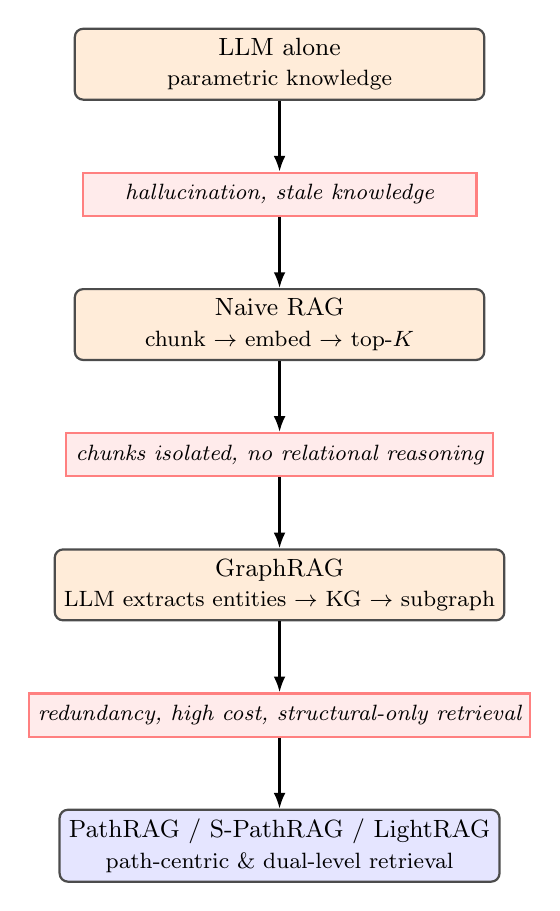
\begin{tikzpicture}[
    node distance=0.9cm,
    box/.style={rectangle, rounded corners=3pt, draw=black!70, thick,
                fill=orange!15, minimum width=5.2cm, minimum height=0.9cm,
                align=center, font=\small},
    gap/.style={rectangle, draw=red!50, thick, fill=red!8,
                minimum width=5cm, minimum height=0.55cm, align=center,
                font=\footnotesize\itshape},
    arr/.style={-{Latex[length=2mm]}, thick}
]
\node[box] (llm) {LLM alone\\\footnotesize parametric knowledge};
\node[gap, below=of llm] (gap1) {hallucination, stale knowledge};
\node[box, below=of gap1] (rag) {Naive RAG\\\footnotesize chunk $\to$ embed $\to$ top-$K$};
\node[gap, below=of rag] (gap2) {chunks isolated, no relational reasoning};
\node[box, below=of gap2] (graph) {GraphRAG\\\footnotesize LLM extracts entities $\to$ KG $\to$ subgraph};
\node[gap, below=of graph] (gap3) {redundancy, high cost, structural-only retrieval};
\node[box, below=of gap3, fill=blue!10] (next) {PathRAG / S-PathRAG / LightRAG\\\footnotesize path-centric \& dual-level retrieval};
\draw[arr] (llm) -- (gap1);
\draw[arr] (gap1) -- (rag);
\draw[arr] (rag) -- (gap2);
\draw[arr] (gap2) -- (graph);
\draw[arr] (graph) -- (gap3);
\draw[arr] (gap3) -- (next);
\end{tikzpicture}
\caption{Architectural progression from LLMs to next-generation graph-based
RAG. Each paradigm emerges as the failure mode of the previous one is
identified. Adapted from \citet{han2025}.}
\label{fig:progression}
\end{figure}

\section{Problem Statement}

Traditional graph-based RAG systems retrieve entire communities or local
neighbourhoods around query-related nodes. This produces prompts that are
rich in information but also saturated with irrelevant content, which
degrades LLM reasoning quality and inflates token cost. The central problem,
as highlighted in recent work \citep{chen2025pathrag} and in the project's
reference video lecture \citep{videoref2026}, is not the \emph{absence} of
information but the \emph{excess} of it. In parallel, purely structural
retrieval methods fail to fully align retrieved paths with query semantics,
and one-shot retrieval leaves no room for refinement when the initial
evidence is insufficient.

This project therefore addresses the following research question:
\begin{quote}
\itshape
How do recent graph-based RAG frameworks---PathRAG, S-PathRAG, and
LightRAG---differ in the way they index knowledge, retrieve evidence, and
interact with the LLM, and what are the practical trade-offs between
retrieval quality, semantic alignment, and computational efficiency?
\end{quote}

\section{Objectives}

\begin{enumerate}[leftmargin=2em,itemsep=2pt]
    \item To study the graph construction and indexing strategies used by
          PathRAG, S-PathRAG, and LightRAG.
    \item To analyse the retrieval pipelines of each framework, focusing on
          path pruning, semantic scoring, and dual-level retrieval.
    \item To compare the three frameworks on redundancy reduction, multi-hop
          reasoning support, and token efficiency.
    \item To identify the conditions under which each framework is most
          suitable for real-world knowledge-intensive question answering.
\end{enumerate}

\section{Scope of the Study}

The scope of this study is limited to graph-based RAG frameworks that operate
on entity--relation knowledge graphs constructed from unstructured text. The
work focuses on methodological comparison and does not attempt a full-scale
empirical benchmark; where quantitative claims are made, they are taken from
the original publications and clearly cited. The study does not cover purely
vector-based RAG, agentic RAG, or multimodal extensions.

\section{Significant Contributions}

\begin{itemize}[leftmargin=2em,itemsep=2pt]
    \item A unified description of PathRAG, S-PathRAG, and LightRAG under a
          common four-stage pipeline.
    \item A structured comparison of their strengths and limitations.
    \item Recommendations on framework selection based on application
          constraints.
\end{itemize}

% ------------------------------------------------------------
\chapter{Rationale}
\label{ch:rationale}

The rationale behind this study stems from the growing gap between the
capability of LLMs and the practical cost of grounding them in large
knowledge bases. Enterprise deployments increasingly require RAG systems
that are simultaneously (i)~accurate over multi-hop questions, (ii)~efficient
in token usage, and (iii)~capable of continuous knowledge updates.

Existing graph-based approaches each solve part of this problem but leave
others open:
\begin{itemize}[leftmargin=2em,itemsep=2pt]
    \item GraphRAG-style community retrieval is thematically rich but
          computationally expensive.
    \item Naive vector RAG is cheap but structurally blind and
          redundancy-prone.
    \item Newer path-centric and dual-level methods promise both structure
          and efficiency, but practitioners lack a clear comparison.
\end{itemize}

A focused comparative study of PathRAG, S-PathRAG, and LightRAG is therefore
timely and directly useful for researchers and engineers selecting a
graph-based RAG architecture. The present work is further motivated by the
reference video lecture on the evolution of graph-based RAG
\citep{videoref2026}, which frames redundancy and hallucination as the two
dominant failure modes that next-generation frameworks must address.

% ------------------------------------------------------------
\chapter{Literature Review}
\label{ch:literature_review}

This chapter traces the architectural progression from plain Large Language
Models, through Naive Retrieval-Augmented Generation, to Graph-based RAG. It
situates the next-generation frameworks (PathRAG, S-PathRAG, LightRAG)
examined in later chapters within this broader lineage. The treatment here
draws heavily on \citet{han2025}'s holistic GraphRAG survey,
\citet{edge2024}'s Microsoft GraphRAG implementation, and \citet{erickson2025}'s
empirical work on knowledge-graph-validated LLM outputs.

\section{Large Language Models}
\label{sec:lit_llm}

\subsection{Architecture and Training}

A Large Language Model is a neural network --- typically based on the
Transformer architecture --- trained on massive corpora to model the
conditional probability of the next token given all preceding tokens
\citep{yang2024}. Through next-token prediction applied at enormous scale
(billions of parameters, trillions of tokens), LLMs develop emergent
capabilities including reasoning \citep{wei2022}, summarisation,
translation, and structured question answering.

The knowledge an LLM possesses is entirely \emph{parametric}, encoded in
frozen weights. At inference time, the model has no mechanism for consulting
external sources or verifying its outputs.

\subsection{Capabilities and Limitations}

Three failure modes are central to motivating RAG \citep{tonmoy2024}:
\begin{itemize}[leftmargin=2em,itemsep=2pt]
    \item \textbf{Hallucination:} confident but factually incorrect outputs.
          Hallucinations split into \emph{intrinsic} (contradicting source
          material) and \emph{extrinsic} (fabricated facts).
    \item \textbf{Knowledge cutoff:} parametric memory is frozen at the
          training date.
    \item \textbf{Lack of verifiability:} the model cannot cite the specific
          source from which a claim originates.
\end{itemize}

\begin{tcolorbox}[colback=blue!5, colframe=blue!45!black, boxrule=0.4pt,
                  title=\textbf{Why hallucination is structural, not incidental}]
\small
LLMs do not retrieve facts --- they interpolate. When asked a question, the
model selects the most probable token sequence under its training
distribution, not the most accurate. In domains where accurate answers are
rare in training data, the distribution assigns high weight to
plausible-sounding but incorrect outputs. RAG and GraphRAG address this by
replacing interpolation with retrieval.
\end{tcolorbox}

\section{Naive Retrieval-Augmented Generation}
\label{sec:lit_naive_rag}

\subsection{The Three-Stage Pipeline}

RAG was introduced by \citet{lewis2020} as a general framework for grounding
LLM generation in retrieved evidence. In its naive form, the pipeline has
three sequential stages \citep{gao2023,fan2024}.

\begin{table}[H]
\centering
\caption{Naive RAG three-stage pipeline.}
\label{tab:naive_rag}
\small
\begin{tabularx}{\textwidth}{@{}lXX@{}}
\toprule
\textbf{Stage} & \textbf{What happens} & \textbf{Mechanism} \\
\midrule
1. Indexing   & Documents are chunked and embedded into a vector space & Chunking + embedding model (BERT, text-embedding-ada) \\
2. Retrieval  & Query is embedded; top-$K$ nearest chunks returned     & Cosine similarity / BM25 over a vector DB \\
3. Generation & Retrieved chunks concatenated into a prompt            & LLM (GPT-4, Llama, etc.) generates answer \\
\bottomrule
\end{tabularx}
\end{table}

\subsection{Strengths and Structural Limitations}

Naive RAG reduces hallucination for single-fact queries and bypasses the
knowledge-cutoff problem. Between 2022 and 2024 it became the de facto
standard for enterprise document Q\&A. However, it has three structural
limitations \citep{han2025,msresearch2024}:
\begin{itemize}[leftmargin=2em,itemsep=2pt]
    \item \textbf{Multi-hop reasoning failure:} queries requiring facts from
          multiple documents connected by a relational path cannot be
          answered by top-$K$ chunk retrieval.
    \item \textbf{Global understanding failure:} holistic questions about
          themes or trends cannot be answered by any finite passage set,
          because the answer is an aggregate property of the whole corpus.
    \item \textbf{No relational structure:} text chunks encode relations
          implicitly, but retrieval operates on surface similarity, not
          logical structure.
\end{itemize}

\section{Graph-Based Retrieval-Augmented Generation (GraphRAG)}
\label{sec:lit_graphrag}

\subsection{Core Concept}

GraphRAG replaces the flat vector store with a \emph{knowledge graph}: a
structured database in which entities (nodes) are connected by typed
relationships (edges). The system retrieves \emph{subgraphs} rather than
passages, enabling multi-hop traversal, explicit reasoning paths, and
answers verifiable against a structured source \citep{han2025,peng2024}.

\subsection{The Five-Component Framework}

\citet{han2025} propose a unified framework in which every GraphRAG system
decomposes into five components.

\begin{table}[H]
\centering
\caption{The five-component GraphRAG framework \citep{han2025}.}
\label{tab:five_component}
\small
\begin{tabularx}{\textwidth}{@{}lXX@{}}
\toprule
\textbf{Component} & \textbf{Function} & \textbf{Key techniques} \\
\midrule
Query Processor   & Parse NL query into graph-compatible form    & NER, relation extraction, query decomposition, query expansion \\
Graph Data Source & Store knowledge as nodes + typed edges       & Explicit (citation links) or implicit (co-occurrence) construction; adjacency or edge lists \\
Retriever         & Fetch relevant subgraphs / paths / nodes     & Heuristic (BFS/DFS); learning-based (GNNs, embeddings); advanced (iterative, agentic) \\
Organiser         & Post-process retrieved graph for generator   & Graph pruning (semantic / syntactic / structural); reranking; verbalisation \\
Generator         & Produce final answer from query + subgraph   & LLM with verbalised graph; embedding-fusion; GNN-based \\
\bottomrule
\end{tabularx}
\end{table}

\subsection{How GraphRAG Is Built Through LLMs}

A critical and often underappreciated feature of modern GraphRAG is that the
LLM is not merely the generator --- it is also the \emph{constructor} of the
knowledge graph. \citet{edge2024} describe the Microsoft GraphRAG
construction pipeline:
\begin{enumerate}[leftmargin=2em,itemsep=2pt]
    \item \textbf{Entity and relationship extraction:} the LLM reads each
          document chunk and identifies entities (with types and
          descriptions) and all pairwise relationships.
    \item \textbf{Knowledge graph assembly:} extracted (entity, relation,
          entity) triples are assembled into an initial graph.
    \item \textbf{Hierarchical clustering:} the Leiden algorithm identifies
          densely connected \emph{communities}.
    \item \textbf{Community summarisation:} the LLM generates natural-language
          summaries of each community.
    \item \textbf{Query-time retrieval:} \emph{local search} (entity
          traversal) for specific queries; \emph{global search} (community
          summaries) for holistic queries.
\end{enumerate}

This creates a feedback loop: the LLM's language understanding is used to
build the very structure that grounds the LLM's future outputs.

\begin{tcolorbox}[colback=orange!5, colframe=orange!70!black, boxrule=0.4pt,
                  title=\textbf{Empirical finding: the ChatBS-NexGen nutrition case study}]
\small
\citet{erickson2025} submitted nutrition prompts to GPT-4o mini and
Llama 3.1-8B for 100 patient records, validating each recommendation against
the FoodKG knowledge graph. Key findings:
(1) Both LLMs recommended high-glycaemic-index foods (GI $\geq 50$) to
diabetic patients, including honey (GI 60), maple syrup (GI 65), rice cake
(GI 85), and watermelon (GI 75).
(2) The global Jaccard similarity index for GPT-4o mini was only $0.05$
across 10 repeated submissions for the same patient, revealing severe
output instability.
(3) FoodKG covered only $36.8\%$ of distinct foods recommended
($47.3\%$ for diabetic-specific recommendations), illustrating the
incompleteness of even well-curated knowledge graphs.
\end{tcolorbox}

\section{Systematic Comparison: LLM, Naive RAG, GraphRAG}
\label{sec:lit_comparison}

\begin{table}[H]
\centering
\caption{Pipeline transformation from Naive RAG to GraphRAG.}
\label{tab:pipeline_transform}
\small
\begin{tabularx}{\textwidth}{@{}lXXX@{}}
\toprule
\textbf{Stage} & \textbf{Naive RAG} & \textbf{GraphRAG} & \textbf{Key difference} \\
\midrule
Input       & User query (text)            & User query (text)                      & Same \\
Indexing    & Chunk $\to$ embed $\to$ VDB  & LLM extracts entities \& relations $\to$ KG & Graph replaces vector store \\
Retrieval   & Top-$K$ cosine similarity    & Entity linking $\to$ traversal / GNN   & Relational paths vs.\ text similarity \\
Organise    & Concatenate chunks           & Prune, rerank, verbalise subgraph      & Structure-aware filtering \\
Generate    & LLM + retrieved text         & LLM + structured subgraph              & Grounded in verified graph facts \\
Output      & Answer (text)                & Answer + citable reasoning path        & Explainability added \\
\bottomrule
\end{tabularx}
\end{table}

\begin{table}[H]
\centering
\caption{Dimension-by-dimension comparison of the three paradigms.}
\label{tab:dimensions}
\small
\begin{tabularx}{\textwidth}{@{}lXXX@{}}
\toprule
\textbf{Dimension} & \textbf{LLM alone} & \textbf{Naive RAG} & \textbf{GraphRAG} \\
\midrule
Knowledge source     & Parametric weights    & Text chunks (vector DB)  & Knowledge graph + text \\
Multi-hop reasoning  & Limited / unreliable  & Poor (chunks isolated)   & Native -- traverses paths \\
Hallucination risk   & High                  & Moderate                 & Low (graph-grounded) \\
Explainability       & Opaque                & Citation-level           & Full relational path \\
Dynamic update       & Requires retraining   & Re-index documents       & Update graph incrementally \\
Consistency          & Variable              & Moderate                 & Structured -- more stable \\
Compute cost         & Low (inference only)  & Moderate                 & Higher (graph build + query) \\
Best use case        & General language      & Simple factual QA        & Complex multi-hop reasoning \\
\bottomrule
\end{tabularx}
\end{table}

\section{Open Research Challenges}
\label{sec:lit_open_challenges}

Despite GraphRAG's advantages, several challenges remain unresolved
\citep{han2025,erickson2025}:
\begin{itemize}[leftmargin=2em,itemsep=2pt]
    \item \textbf{Knowledge-graph completeness:} as in the FoodKG case, even
          curated graphs cover only a fraction of the entities mentioned in
          real queries.
    \item \textbf{Response consistency:} Jaccard-similarity scores as low as
          $0.05$ across repeated identical prompts reveal that even
          graph-augmented pipelines are not reproducible without additional
          controls.
    \item \textbf{Query formulation:} translating natural language into
          graph-query form (Cypher, SPARQL, GQL) remains difficult,
          particularly for non-expert users.
    \item \textbf{Trustworthiness and safety:} relational structure can leak
          private information via neighbour traversal, raising new privacy
          and fairness concerns.
\end{itemize}

\section{Position of this Report}
\label{sec:lit_position}

The literature reviewed above establishes the \emph{foundations} of
graph-based RAG up to and including Microsoft-style community GraphRAG
\citep{edge2024,han2025}. The present report picks up where this literature
ends: it examines three \emph{next-generation} graph-based RAG frameworks
--- PathRAG, S-PathRAG, and LightRAG --- that explicitly target the
computational-cost and redundancy limitations of community-based GraphRAG.
The connection from this chapter to the rest of the report is visualised in
Figure~\ref{fig:progression}.

\section{A Practical Observation}
\label{sec:practical_observation}

A secondary observation runs alongside the main comparative study. In all
three frameworks examined in this report, the LLM plays a dual role: it
\emph{constructs} the knowledge graph via entity and relation extraction,
and later \emph{queries} the graph at answer-generation time. The original
papers describe this dual role but treat the LLM component as
interchangeable; none of them study how the specific LLM used for
construction affects the quality of the resulting graph. While
implementing a LightRAG-style pipeline for this study
(Chapter~\ref{ch:methodology}), we observed that substituting different
LLMs into the extraction step produces visibly different knowledge graphs
on identical input. Results of this small side-observation are reported
in Section~\ref{sec:empirical_observation}.

% ------------------------------------------------------------
\chapter{Research Envisaged, Objectives and Plan of Work}
\label{ch:research_plan}

\section{Status of the Problem}

Graph-based RAG is an active area of research. Three directions have emerged
as particularly promising: path-centric retrieval (PathRAG), semantic-aware
iterative retrieval (S-PathRAG), and lightweight dual-level retrieval
(LightRAG). Each addresses different failure modes of earlier RAG systems,
but no consolidated comparison exists that places them side by side in terms
of methodology, cost, and reasoning capability.

\section{Hypotheses}

The project is guided by the following working hypotheses:
\begin{itemize}[leftmargin=2em,itemsep=2pt]
    \item \textbf{H1.} Path-centric retrieval (PathRAG) reduces prompt
          redundancy compared with neighbourhood- or community-based retrieval
          without sacrificing answer quality.
    \item \textbf{H2.} Introducing semantic-aware scoring and iterative
          refinement (S-PathRAG) improves multi-hop reasoning and reduces
          hallucinations relative to purely structural retrieval.
    \item \textbf{H3.} Dual-level retrieval (LightRAG) achieves substantially
          lower token and API cost than community-based GraphRAG while
          retaining retrieval accuracy.
\end{itemize}

\section{Research Objectives}

\begin{enumerate}[leftmargin=2em,itemsep=2pt]
    \item Characterise the indexing graph, retrieval pipeline, and
          generation strategy of each framework.
    \item Compare the three frameworks along the axes of redundancy,
          semantic alignment, multi-hop reasoning, and efficiency.
    \item Summarise the trade-offs and provide deployment-oriented
          recommendations.
\end{enumerate}

\section{Plan of Work}

The project is organised in four phases:
\begin{enumerate}[leftmargin=2em,itemsep=2pt]
    \item \textbf{Study phase:} review of the original PathRAG, S-PathRAG,
          and LightRAG publications and associated materials.
    \item \textbf{Analysis phase:} decomposition of each framework into a
          common four-stage pipeline (graph construction, indexing,
          retrieval, generation).
    \item \textbf{Comparison phase:} cross-framework analysis using
          qualitative criteria and quantitative claims reported in the
          source papers.
    \item \textbf{Reporting phase:} consolidation of findings, trade-off
          discussion, and recommendations.
\end{enumerate}

% ------------------------------------------------------------
\chapter{Data Preparation}
\label{ch:data_preparation}

Since this report is a comparative methodological study, ``data preparation''
here refers to the process by which each framework converts a raw text
corpus into a structured knowledge graph suitable for retrieval.

\section{Corpus-to-Graph Construction}

All three frameworks begin with an unstructured text corpus and use an LLM
to extract structured knowledge. The shared steps are:
\begin{enumerate}[leftmargin=2em,itemsep=2pt]
    \item \textbf{Chunking:} source documents are split into semantically
          coherent chunks.
    \item \textbf{Entity and relation extraction:} an LLM extracts
          Subject--Predicate--Object (SPO) triplets from each chunk
          \citep{guo2025lightrag}.
    \item \textbf{Node and edge creation:} entities become nodes and
          relationships become edges; each is annotated with a textual
          description.
    \item \textbf{Embedding:} node, edge, and chunk embeddings are computed
          and stored for similarity search.
\end{enumerate}

\section{Storage Layout}

LightRAG uses a three-tier storage strategy that is representative of the
class as a whole \citep{guo2025lightrag}:
\begin{itemize}[leftmargin=2em,itemsep=2pt]
    \item \textbf{KV\_STORAGE:} LLM response caches, text chunks, and
          document metadata.
    \item \textbf{VECTOR\_STORAGE:} high-dimensional embeddings of entities,
          relations, and chunks.
    \item \textbf{GRAPH\_STORAGE:} topology of the entity--relationship
          network (e.g., Neo4j or a local graph structure).
\end{itemize}

\section{Framework-Specific Preparation}

\begin{itemize}[leftmargin=2em,itemsep=2pt]
    \item \textbf{PathRAG} pre-computes textual descriptions for each node
          and edge so that retrieved paths can be serialised into
          natural-language evidence \citep{chen2025pathrag}.
    \item \textbf{S-PathRAG} augments the graph with learned embeddings
          produced by a contrastive path encoder, enabling semantic
          similarity scoring at retrieval time \citep{fu2026spathrag}.
    \item \textbf{LightRAG} generates ``profiles'' for each node and edge as
          key--value pairs, where keys are optimised for rapid search and
          values summarise contextual role \citep{guo2025lightrag}.
\end{itemize}

\begin{table}[H]
    \centering
    \caption{Comparison of graph construction choices across the three
             frameworks.}
    \label{tab:graph_construction}
    \small
    \begin{tabularx}{\textwidth}{@{}lXXX@{}}
        \toprule
        \textbf{Aspect} & \textbf{PathRAG} & \textbf{S-PathRAG} & \textbf{LightRAG} \\
        \midrule
        Primary unit     & Relational path        & Semantic-aware path         & Entity + dual-level index \\
        Node/edge profile& Textual descriptions   & Latent embeddings + text    & Key--value profiles \\
        Index focus      & Structural importance  & Semantic + structural       & Local + global summaries \\
        Update mode      & Re-indexing            & Re-indexing                 & Incremental \\
        \bottomrule
    \end{tabularx}
\end{table}

% ------------------------------------------------------------
\chapter{Methodology}
\label{ch:methodology}

This chapter details the retrieval and generation methodologies of each of
the three frameworks under study.

\section{PathRAG: Path-Based Retrieval}

PathRAG shifts retrieval from a \emph{node-centric} paradigm to a
\emph{path-centric} paradigm \citep{chen2025pathrag}. Rather than returning
all nodes or subgraphs related to a query, it retrieves a small number of
structured relational paths between query-relevant entities.

\subsection{Node Retrieval}
The query is processed by an LLM to extract keywords, which are then embedded
and compared against node embeddings using cosine similarity. The
top-matching nodes form the \emph{anchor set} for path search.

\subsection{Path Retrieval with Flow-Based Pruning}
Between anchor nodes, candidate paths are enumerated. To avoid combinatorial
explosion, PathRAG applies a \emph{flow-based pruning} mechanism governed by
three principles:
\begin{itemize}[leftmargin=2em,itemsep=2pt]
    \item \textbf{Importance propagation:} relevance is propagated through
          the graph starting from query-related nodes.
    \item \textbf{Decay with distance:} nodes farther from the source
          receive lower importance.
    \item \textbf{Early pruning:} paths with low accumulated importance are
          discarded before full expansion.
\end{itemize}

\subsection{Path Scoring and Answer Generation}
Each surviving path is assigned a reliability score based on node importance
and the structural strength of the connection. The top-$K$ paths are
selected, linearised into natural-language evidence, and arranged
strategically in the prompt to maximise LLM attention on high-value
information.

\section{S-PathRAG: Semantic-Aware Iterative Retrieval}

S-PathRAG extends PathRAG with semantic awareness and an iterative refinement
loop \citep{fu2026spathrag}.

\subsection{Semantic-Aware Path Retrieval}
Paths are scored using both structural plausibility and semantic similarity
to the query, so that retrieved evidence aligns with user intent rather than
graph topology alone.

\subsection{Hybrid Path Enumeration}
Candidate paths are generated using a combination of shortest-path search,
beam-based expansion, and random-walk exploration, balancing coverage
against efficiency.

\subsection{Differentiable Path Scoring and Verification}
A learning-based scoring module contains:
\begin{itemize}[leftmargin=2em,itemsep=2pt]
    \item a \emph{path scorer} that ranks paths;
    \item a \emph{contrastive path encoder} that produces semantic
          representations;
    \item a \emph{verifier} that filters out paths not supported by the
          knowledge graph.
\end{itemize}
The verifier is the key mechanism for reducing hallucinated or weakly
grounded paths.

\subsection{Latent Path Injection}
Rather than serialising paths into long textual prompts, S-PathRAG encodes
them into latent embeddings that are injected into the LLM via
cross-attention. This preserves structured information while reducing token
consumption.

\subsection{Iterative Retrieval (Neural-Socratic Graph Dialogue)}
The LLM emits diagnostic feedback indicating uncertainty or missing
information. The framework uses this signal to update retrieval, producing a
closed-loop refinement process in contrast to the one-shot retrieval of
PathRAG.

\section{LightRAG: Dual-Level Lightweight Retrieval}

LightRAG is designed as a \emph{lightweight} alternative to community-based
GraphRAG \citep{guo2025lightrag}, sitting between naive vector RAG and heavy
graph traversal.

\subsection{Graph-Based Text Indexing and Profiling}
LightRAG uses an LLM to extract SPO triplets from the corpus and generates
key--value profiles for every node and edge. Keys are optimised for rapid
lookup; values summarise contextual role.

\subsection{Dual-Level Retrieval}
At query time, LightRAG performs retrieval at two granularities
simultaneously:
\begin{itemize}[leftmargin=2em,itemsep=2pt]
    \item \textbf{Low-level retrieval:} targets specific entities and direct
          attributes, supporting precise ``who/what/when'' questions.
    \item \textbf{High-level retrieval:} targets global themes and
          cross-document concepts, supporting ``why/how'' reasoning.
\end{itemize}
A \emph{hybrid (mix) mode} combines both levels to provide unified
contextual grounding.

\subsection{Incremental Updating}
Unlike frameworks requiring full re-indexing on knowledge updates, LightRAG
supports incremental insertion of new entities and relationships, making it
suitable for evolving corpora.

\section{Software and Tools}

The methodological comparison draws on the reference implementations and
descriptions provided by the original authors of PathRAG, S-PathRAG, and
LightRAG. Alongside this comparison, a LightRAG-style pipeline was
implemented to provide hands-on grounding
(Section~\ref{sec:implementation}).

\section{LightRAG-Style Implementation}
\label{sec:implementation}

To develop concrete familiarity with graph-based RAG, a LightRAG-style
extraction-and-indexing pipeline was implemented from first principles,
following the architectural outline of \citet{guo2025lightrag}. The
pipeline replicates the core indexing step shared by PathRAG, S-PathRAG,
and LightRAG --- namely, LLM-driven entity and relation extraction from
text chunks --- and persists the resulting knowledge graph to disk as a
GraphML file.

\subsection{Corpus and Gold Reference}

The pipeline was exercised on a domain-appropriate corpus of \textbf{ten
Wikipedia articles} spanning four entity types in cancer drug-target
research:

\begin{table}[H]
\centering
\caption{Composition of the cancer drug-target corpus used to exercise the
implementation.}
\label{tab:corpus}
\small
\begin{tabularx}{\textwidth}{@{}lXl@{}}
\toprule
\textbf{Entity type} & \textbf{Articles} & \textbf{Count} \\
\midrule
Cancer (disease) & Breast cancer; Chronic myeloid leukemia; Melanoma & 3 \\
Drug             & Trastuzumab; Imatinib; Pembrolizumab               & 3 \\
Gene / target    & BRCA1; EZH2                                        & 2 \\
Pathway          & Apoptosis; p53 (TP53)                              & 2 \\
\bottomrule
\end{tabularx}
\end{table}

The corpus was tokenised into 148 chunks of approximately 500 tokens each.
A small gold reference graph (60 human-validated triples) was annotated
from a single chunk in the EZH2 article --- specifically the
``Inhibitors'' section, which is the source of the canonical
\emph{tazemetostat\,$\to$\,epithelioid sarcoma} multi-hop example used in
the graph-RAG literature \citep{han2025}.

\subsection{Software Stack}

\begin{itemize}[leftmargin=2em,itemsep=2pt]
    \item Python 3.12 as the base language.
    \item Provider-native SDKs (OpenAI Python SDK; Anthropic via the
          Claude Code CLI backend; Groq via OpenAI-compatible API) for
          LLM-driven extraction.
    \item \texttt{tiktoken} for tokenisation-aware corpus chunking.
    \item NetworkX \citep{networkx2008} for graph construction, topology
          analysis, and GraphML export.
    \item Pandas and scikit-learn for metrics; Matplotlib for plotting.
    \item No third-party RAG framework (LangChain, LlamaIndex, the
          LightRAG reference library) is used, so that the pipeline is
          transparent and each stage is directly inspectable.
\end{itemize}

\subsection{Extraction Prompt}

For each chunk, the selected LLM receives a structured system prompt
requesting JSON output containing \texttt{(subject, predicate, object)}
triples together with entity types and verbatim evidence spans. The same
prompt is used for every LLM evaluated. Extracted triples from all chunks
are aggregated into a single directed multigraph for downstream analysis.

\section{Evaluation Criteria}

The three frameworks are compared on:
\begin{itemize}[leftmargin=2em,itemsep=2pt]
    \item \textbf{Retrieval quality:} precision and coverage of retrieved
          evidence.
    \item \textbf{Redundancy:} token overlap and noise in the prompt.
    \item \textbf{Multi-hop reasoning:} ability to chain evidence across
          multiple relations.
    \item \textbf{Hallucination rate:} frequency of unsupported answers.
    \item \textbf{Efficiency:} API calls, token consumption, and end-to-end
          latency.
\end{itemize}

\begin{figure}[H]
\centering
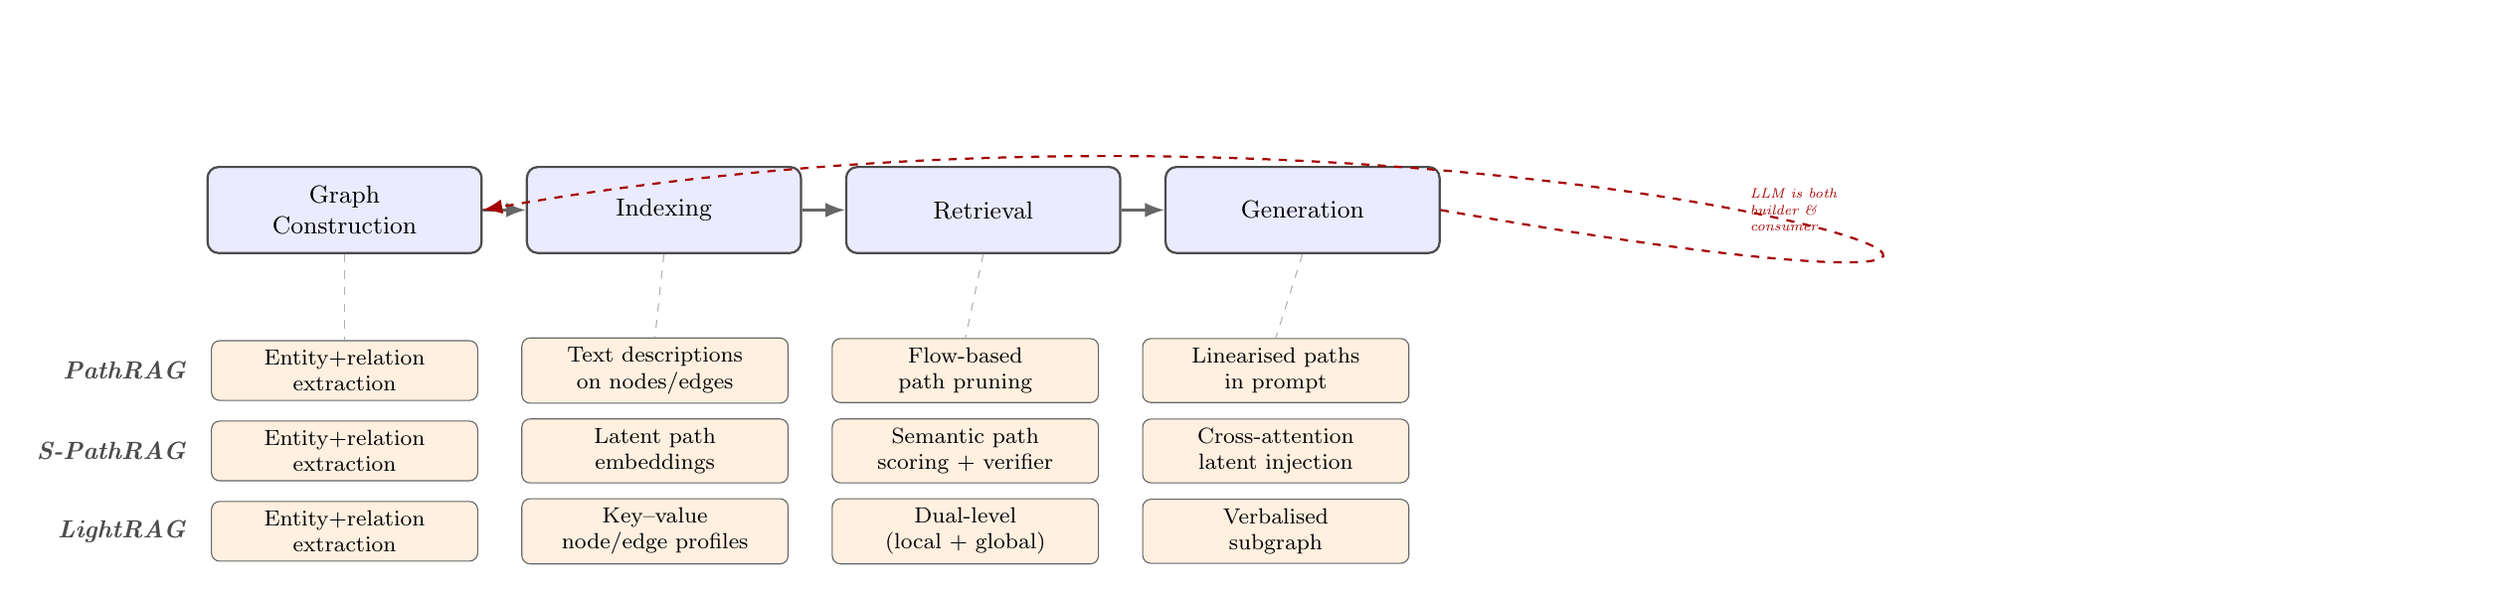
\begin{tikzpicture}[
    node distance=0.55cm,
    stage/.style={rectangle, rounded corners=4pt, draw=black!70, thick,
                  fill=blue!8, minimum width=3.5cm, minimum height=1.1cm,
                  align=center, font=\small},
    framework/.style={rectangle, rounded corners=3pt, draw=black!60,
                      fill=orange!12, minimum width=3.4cm, minimum height=0.75cm,
                      align=center, font=\footnotesize},
    arr/.style={-{Latex[length=2.5mm]}, thick, black!60},
    grouplabel/.style={font=\small\itshape, text=black!70},
]

% Top row: four pipeline stages
\node[stage] (gc)  {Graph\\Construction};
\node[stage, right=of gc]  (ix) {Indexing};
\node[stage, right=of ix]  (rt) {Retrieval};
\node[stage, right=of rt]  (gn) {Generation};
\draw[arr] (gc) -- (ix);
\draw[arr] (ix) -- (rt);
\draw[arr] (rt) -- (gn);

% PathRAG row
\node[framework, below=1.1cm of gc]
    (p_gc) {Entity+relation\\extraction};
\node[framework, right=of p_gc]
    (p_ix) {Text descriptions\\on nodes/edges};
\node[framework, right=of p_ix]
    (p_rt) {Flow-based\\path pruning};
\node[framework, right=of p_rt]
    (p_gn) {Linearised paths\\in prompt};
\node[grouplabel, left=0.2cm of p_gc]
    (plab) {\textbf{PathRAG}};

% S-PathRAG row
\node[framework, below=0.25cm of p_gc]
    (s_gc) {Entity+relation\\extraction};
\node[framework, right=of s_gc]
    (s_ix) {Latent path\\embeddings};
\node[framework, right=of s_ix]
    (s_rt) {Semantic path\\scoring + verifier};
\node[framework, right=of s_rt]
    (s_gn) {Cross-attention\\latent injection};
\node[grouplabel, left=0.2cm of s_gc]
    (slab) {\textbf{S-PathRAG}};

% LightRAG row
\node[framework, below=0.25cm of s_gc]
    (l_gc) {Entity+relation\\extraction};
\node[framework, right=of l_gc]
    (l_ix) {Key--value\\node/edge profiles};
\node[framework, right=of l_ix]
    (l_rt) {Dual-level\\(local + global)};
\node[framework, right=of l_rt]
    (l_gn) {Verbalised\\subgraph};
\node[grouplabel, left=0.2cm of l_gc]
    (llab) {\textbf{LightRAG}};

% Dotted guides from top stages to rows
\draw[dashed, black!30] (gc.south) -- (p_gc.north);
\draw[dashed, black!30] (ix.south) -- (p_ix.north);
\draw[dashed, black!30] (rt.south) -- (p_rt.north);
\draw[dashed, black!30] (gn.south) -- (p_gn.north);

% LLM-as-constructor highlight (feedback loop arrow)
\draw[arr, red!65!black, dashed]
    (gn.east) to[out=-10, in=10, looseness=2.8]
    node[right=2pt, font=\tiny\itshape, text=red!65!black, align=left]
    {LLM is both\\builder \&\\consumer} (gc.east);

\end{tikzpicture}
\caption{Unified four-stage view of the PathRAG, S-PathRAG, and LightRAG
         pipelines. All three share the top row (graph construction
         $\rightarrow$ indexing $\rightarrow$ retrieval $\rightarrow$
         generation) but differ in the specific techniques used at each
         stage (orange boxes). The dashed red arrow indicates the
         LLM-as-graph-constructor feedback loop.}
\label{fig:pipeline}
\end{figure}

% ------------------------------------------------------------
\chapter{Results and Discussion}
\label{ch:results}

\section{Comparative Findings}

\subsection{Retrieval Paradigm}
PathRAG is the first of the three to formalise \emph{path-centric}
retrieval. By propagating importance scores and pruning early, it
consistently produces shorter, denser evidence than community- or
neighbourhood-based retrieval \citep{chen2025pathrag}. S-PathRAG retains the
path-centric view but enriches it with semantic alignment, which is critical
for queries whose surface form does not match graph topology
\citep{fu2026spathrag}. LightRAG takes a different approach: rather than
choosing a single retrieval granularity, it performs retrieval at two levels
simultaneously \citep{guo2025lightrag}.

\subsection{Redundancy and Token Usage}
All three frameworks aim to reduce the prompt bloat associated with earlier
graph-based RAG. PathRAG's flow-based pruning removes irrelevant branches
before serialisation. S-PathRAG goes further by replacing long textual paths
with latent embeddings injected via cross-attention, cutting token use while
preserving structure. LightRAG reports the largest absolute gains against
GraphRAG: up to a $90\%$ reduction in API calls and up to $6000\times$
reduction in token consumption for specific datasets, while maintaining or
exceeding retrieval accuracy \citep{guo2025lightrag}.

\subsection{Multi-Hop Reasoning and Hallucination Control}
PathRAG supports multi-hop reasoning implicitly through the structure of
retrieved paths, but has no explicit hallucination filter. S-PathRAG
introduces a verifier module that rejects plausible-looking but unsupported
paths, and an iterative loop (``Neural-Socratic Graph Dialogue'') that
refines retrieval based on LLM feedback \citep{fu2026spathrag}. LightRAG
handles multi-hop questions through its hybrid mode, where high-level themes
are combined with low-level entity facts to form a more complete context.

\subsection{Domain Specialisation}
LightRAG has seen rapid adoption in specialised domains. In geosciences, a
LightRAG-based GeoGPT pipeline achieved an F1-score of $0.835$ for entity
extraction, surpassing general-purpose models by $53$--$78\%$ in
remote-sensing benchmarks \citep{geogpt2026}. In clinical settings,
Co-MedGraphRAG uses LightRAG's dual-level retrieval to generate personalised,
evidence-based responses at low latency \citep{limedgraph2026}.

\section{Summary Comparison}

\begin{table}[H]
    \centering
    \caption{Qualitative comparison of PathRAG, S-PathRAG, and LightRAG.}
    \label{tab:qualitative}
    \small
    \begin{tabularx}{\textwidth}{@{}lXXX@{}}
        \toprule
        \textbf{Criterion} & \textbf{PathRAG} & \textbf{S-PathRAG} & \textbf{LightRAG} \\
        \midrule
        Retrieval unit        & Relational path         & Semantic-aware path        & Dual-level (entity + theme) \\
        Pruning strategy      & Flow-based importance   & Learned scoring + verifier & Profile-guided lookup \\
        Semantic alignment    & Structural only         & Structural + semantic      & Embedding-based \\
        Iterative refinement  & No (one-shot)           & Yes (Socratic loop)        & No (one-shot) \\
        Hallucination control & None explicit           & Verifier module            & Implicit (dual-grounding) \\
        Token efficiency      & High                    & Very high (latent inj.)    & Very high ($6000\times$) \\
        Update mode           & Re-indexing             & Re-indexing                & Incremental \\
        Best suited for       & Short multi-hop QA      & Complex multi-hop QA       & Real-time, large-scale QA \\
        \bottomrule
    \end{tabularx}
\end{table}

\begin{table}[H]
    \centering
    \caption{Reported efficiency gains of LightRAG versus community-based
             GraphRAG \citep{guo2025lightrag}.}
    \label{tab:efficiency}
    \small
    \begin{tabular}{@{}lc@{}}
        \toprule
        \textbf{Metric}           & \textbf{LightRAG vs.\ GraphRAG} \\
        \midrule
        API calls (per query)     & up to $90\%$ fewer \\
        Token consumption         & up to $6000\times$ lower \\
        Retrieval accuracy        & matched or exceeded \\
        \bottomrule
    \end{tabular}
\end{table}

\section{Discussion}

The three frameworks are best viewed as complementary rather than strictly
competing:
\begin{itemize}[leftmargin=2em,itemsep=2pt]
    \item \textbf{PathRAG} is a strong baseline when the priority is clean,
          structured evidence and the corpus is moderate in size.
    \item \textbf{S-PathRAG} is preferable when queries are semantically
          rich, multi-hop, or prone to hallucination, and when the additional
          cost of training the scorer/verifier is acceptable.
    \item \textbf{LightRAG} is the most attractive choice when deployment
          constraints---API cost, latency, incremental updates---dominate
          the design space.
\end{itemize}

A consistent theme across all three is the rejection of ``more is better''
retrieval. The contribution of recent graph-based RAG research is to
demonstrate that \emph{selecting less, more carefully} yields better LLM
reasoning.

\section{Observation: Effect of Extraction LLM on Graph Quality}
\label{sec:empirical_observation}

While implementing the LightRAG-style pipeline described in
Section~\ref{sec:implementation}, we ran the same extraction prompt over
the same 148-chunk cancer corpus under five different extraction LLMs and
compared the resulting graphs against the 60-triple gold reference.
Precision, recall, and F1 in Table~\ref{tab:empirical_quality} are
reported on the gold chunk only, so that each model is evaluated against
identically-sized ground truth.

\begin{table}[H]
\centering
\caption{Extraction quality of five LLMs on the gold reference chunk.
Strict F1 counts a prediction as correct only if the entire
(subject, predicate, object) triple matches the gold after
case/whitespace normalisation; lenient F1 counts entity pairs regardless
of predicate phrasing.}
\label{tab:empirical_quality}
\small
\begin{tabularx}{\textwidth}{@{}lXXXXX@{}}
\toprule
\textbf{LLM} & \textbf{Provider} & \textbf{Precision} & \textbf{Recall} & \textbf{Strict F1} & \textbf{Lenient F1} \\
\midrule
Claude Sonnet 4.6 & Anthropic & 0.58 & 0.30 & \textbf{0.40} & 0.48 \\
Claude Opus 4.6   & Anthropic & 0.45 & 0.32 & 0.37          & 0.45 \\
GPT-5 mini        & OpenAI    & 0.29 & 0.20 & 0.24          & 0.27 \\
Llama 3.3 70B     & Groq      & 0.57 & 0.13 & 0.22          & 0.28 \\
Llama 3.1 8B      & Groq      & 0.05 & 0.02 & 0.03          & 0.08 \\
\bottomrule
\end{tabularx}
\end{table}

\begin{table}[H]
\centering
\caption{Full-corpus graph topology by extraction LLM. ``\#Triples'' is
the total number of extracted triples over the 148-chunk corpus;
``\#Components'' is the number of weakly-connected components in the
resulting multigraph.}
\label{tab:empirical_topology}
\small
\begin{tabularx}{\textwidth}{@{}lXXXX@{}}
\toprule
\textbf{LLM} & \textbf{\#Triples} & \textbf{\#Nodes} & \textbf{\#Edges} & \textbf{\#Components} \\
\midrule
Claude Sonnet 4.6 & 2,926 & 2,130 & 2,926 & 85 \\
Claude Opus 4.6   & 3,155 & 2,348 & 3,103 & 105 \\
GPT-5 mini        & 4,305 & 4,315 & 4,305 & 387 \\
Llama 3.3 70B     & 1,730 & 1,513 & 1,730 & 268 \\
Llama 3.1 8B      & 2,272 & 1,961 & 2,272 & 273 \\
\bottomrule
\end{tabularx}
\end{table}

\begin{table}[H]
\centering
\caption{Pairwise entity Jaccard overlap between extraction LLMs on the
full corpus. A value of 1.00 indicates identical entity sets; lower
values indicate the models extracted different entities from the same
text.}
\label{tab:empirical_jaccard}
\small
\begin{tabularx}{\textwidth}{@{}lXXXXX@{}}
\toprule
 & \textbf{C.\ Sonnet} & \textbf{C.\ Opus} & \textbf{GPT-5 mini} & \textbf{L.\ 70B} & \textbf{L.\ 8B} \\
\midrule
Claude Sonnet 4.6 & 1.00 & 0.25 & 0.15 & 0.36 & 0.23 \\
Claude Opus 4.6   & 0.25 & 1.00 & 0.02 & 0.21 & 0.14 \\
GPT-5 mini        & 0.15 & 0.02 & 1.00 & 0.17 & 0.16 \\
Llama 3.3 70B     & 0.36 & 0.21 & 0.17 & 1.00 & 0.30 \\
Llama 3.1 8B      & 0.23 & 0.14 & 0.16 & 0.30 & 1.00 \\
\bottomrule
\end{tabularx}
\end{table}

Three patterns stand out. First, the \textbf{Claude family dominates
extraction quality} --- Claude Sonnet~4.6 achieves the highest strict F1
(0.40) and Claude Opus~4.6 the highest recall (0.32), with both
substantially ahead of the Groq-hosted Llamas on the same corpus.
Second, \textbf{graph topology varies by an order of magnitude across
LLMs} given the same input: GPT-5 mini produces roughly 2.5$\times$ as
many triples as Llama 3.3 70B, suggesting very different notions of
``what counts as a relation''. Third, \textbf{cross-LLM entity overlap
is low}: even the most-similar pair (Claude Sonnet and Llama 3.3 70B)
share only 36\% of extracted entities, and the least-similar pair (GPT-5
mini and Claude Opus) share just 2\%. The same text produces visibly
different knowledge graphs depending on which model reads it.

These results are an incidental observation from the implementation work,
not a fully-controlled experiment. In particular, the strict-match
metric is unforgiving of paraphrase (e.g.\ \emph{``inhibits EZH2''}
versus \emph{``suppresses EZH2 activity''} score as a miss), which is
one reason lenient F1 runs roughly 1.5--2$\times$ higher than strict F1.
The finding of substantive inter-LLM variation is nonetheless consistent
across all three views: quality, topology, and entity overlap. A more
rigorous evaluation --- larger gold reference, multiple prompt variants,
semantic-similarity matching --- is left for future work
(Section~\ref{sec:future_work}).

\section{Limitations}

\begin{itemize}[leftmargin=2em,itemsep=2pt]
    \item PathRAG is structure-driven, and some selected paths may not align
          with query meaning. Retrieval is one-shot and there is no
          mechanism to filter hallucinated paths \citep{chen2025pathrag}.
    \item S-PathRAG introduces learning components (contrastive encoder,
          verifier) that require training data and compute, which may not
          be available in all deployments.
    \item LightRAG's dual-level retrieval is efficient but less expressive
          for deep chains of reasoning compared with dedicated path-based
          methods.
    \item The empirical observation in
          Section~\ref{sec:empirical_observation} is based on a single
          60-triple gold chunk, one extraction prompt variant, and a
          small set of five LLMs. It is directional, not definitive.
\end{itemize}

% ------------------------------------------------------------
\chapter{Summary and Conclusion}
\label{ch:conclusion}

\section{Summary}

This report has presented a comparative study of three recent graph-based
Retrieval-Augmented Generation frameworks: PathRAG, S-PathRAG, and LightRAG.
Each was decomposed into a common pipeline of graph construction, indexing,
retrieval, and generation, and their mechanisms were contrasted in terms of
retrieval paradigm, redundancy reduction, semantic alignment, multi-hop
reasoning, and efficiency.

\section{Conclusions}

\begin{itemize}[leftmargin=2em,itemsep=2pt]
    \item Path-centric retrieval, as introduced by \textbf{PathRAG}, is an
          effective strategy for eliminating redundant information from
          graph-based RAG prompts.
    \item \textbf{S-PathRAG} advances the state of the art by integrating
          semantic-aware scoring, latent path injection, and an iterative
          Neural-Socratic retrieval loop, which together address the
          hallucination and one-shot-retrieval limitations of PathRAG.
    \item \textbf{LightRAG} achieves the strongest efficiency profile
          through dual-level retrieval and incremental updating, with
          reported reductions of up to $90\%$ in API calls and up to
          $6000\times$ in token consumption relative to community-based
          GraphRAG.
    \item The three frameworks are complementary: framework selection
          should be driven by the application's priorities across reasoning
          depth, semantic complexity, and deployment cost.
\end{itemize}

\section{Scope for Future Work}
\label{sec:future_work}

\begin{itemize}[leftmargin=2em,itemsep=2pt]
    \item \textbf{Hybrid architectures:} combining LightRAG's dual-level
          retrieval with S-PathRAG's semantic verifier to obtain both
          efficiency and reliability.
    \item \textbf{Incremental real-time updates:} extending path-based
          methods to evolving knowledge graphs without full re-indexing.
    \item \textbf{Multimodal RAG:} generalising these frameworks to unified
          graphs containing text, tabular, and visual entities.
    \item \textbf{On-device inference:} leveraging the lightweight nature of
          LightRAG for edge deployments.
    \item \textbf{Empirical benchmarking:} a direct head-to-head evaluation
          of PathRAG, S-PathRAG, and LightRAG on standard multi-hop QA
          benchmarks.
    \item \textbf{LLM-substitution effects on graph quality:} following on
          from the observation in
          Section~\ref{sec:empirical_observation}, a fuller study would
          expand the gold reference beyond one chunk, add semantic
          similarity-based matching to handle paraphrase, sweep prompt
          variants, and include closed-source flagships such as GPT-5 and
          Gemini Pro at full corpus scale.
\end{itemize}

% =============================================================
%  REFERENCES
% =============================================================
\clearpage
\phantomsection
\addcontentsline{toc}{chapter}{References}

\begin{thebibliography}{99}
\setlength{\itemsep}{4pt}

\bibitem[Erickson et~al.(2025)]{erickson2025}
Erickson, J.\,S., Santos, H., Pinheiro, V., McCusker, J.\,P., \& McGuinness,
D.\,L., 2025. LLM experimentation through knowledge graphs: towards
improved management, repeatability, and verification. \textit{Web
Semantics: Science, Services and Agents on the World Wide Web}, 85,
100853.

\bibitem[Fan et~al.(2024)]{fan2024}
Fan, W., Ding, Y., Ning, L., Wang, S., Li, H., Yin, D., Chua, T.-S., \& Li,
Q., 2024. A survey on RAG meeting LLMs: towards retrieval-augmented large
language models. In \textit{Proc.\ 30th ACM SIGKDD Conference on Knowledge
Discovery and Data Mining}, 6491--6501.

\bibitem[Gao et~al.(2023)]{gao2023}
Gao, Y., Xiong, Y., Gao, X., Jia, K., Pan, J., Bi, Y., Dai, Y., Sun, J., \&
Wang, H., 2023. Retrieval-augmented generation for large language models: a
survey. arXiv:2312.10997.

\bibitem[Han et~al.(2025)]{han2025}
Han, H., Wang, Y., Shomer, H., Guo, K., Ding, J., Lei, Y., Halappanavar, M.,
Rossi, R.\,A., Mukherjee, S., Tang, X., He, Q., Hua, Z., Long, B., Zhao, T.,
Shah, N., Javari, A., Xia, Y., \& Tang, J., 2025.
\textit{Retrieval-Augmented Generation with Graphs (GraphRAG).}
arXiv:2501.00309.

\bibitem[Kau et~al.(2024)]{kau2024}
Kau, A., He, X., Nambissan, A., Astudillo, A., Yin, H., \& Aryani, A., 2024.
Combining knowledge graphs and large language models. arXiv:2407.06564.

\bibitem[Microsoft Research(2024)]{msresearch2024}
Microsoft Research, 2024. \textit{GraphRAG: Unlocking LLM discovery on
narrative private data.} Microsoft Research Blog, 2 April 2024.
\url{https://www.microsoft.com/en-us/research/blog/graphrag-unlocking-llm-discovery-on-narrative-private-data/}.

\bibitem[Peng et~al.(2024)]{peng2024}
Peng, B., Zhu, Y., Liu, Y., Bo, X., Shi, H., Hong, C., Zhang, Y., \& Tang,
S., 2024. Graph retrieval-augmented generation: a survey.
arXiv:2408.08921.

\bibitem[Tonmoy et~al.(2024)]{tonmoy2024}
Tonmoy, S.\,M., Zaman, S.\,M., Jain, V., Rani, A., Rawte, V., Chadha, A., \&
Das, A., 2024. A comprehensive survey of hallucination mitigation
techniques in large language models. arXiv:2401.01313.

\bibitem[Wei et~al.(2022)]{wei2022}
Wei, J., Wang, X., Schuurmans, D., Bosma, M., Ichter, B., Xia, F., Chi,
E.\,H., Le, Q.\,V., \& Zhou, D., 2022. Chain-of-thought prompting elicits
reasoning in large language models. In \textit{Proc.\ 36th NeurIPS}.

\bibitem[Yang et~al.(2024)]{yang2024}
Yang, J., Jin, H., Tang, R., Han, X., Feng, Q., Jiang, H., Zhong, S., Yin,
B., \& Hu, X., 2024. Harnessing the power of LLMs in practice: a survey on
ChatGPT and beyond. \textit{ACM Transactions on Knowledge Discovery from
Data}, 18(6), 160:1--160:32.

\bibitem[Zhao et~al.(2024)]{zhao2024}
Zhao, P., Zhang, H., Yu, Q., Wang, Z., Geng, Y., Fu, F., Yang, L., Zhang,
W., \& Cui, B., 2024. Retrieval-augmented generation for AI-generated
content: a survey. arXiv:2402.19473.

\bibitem[Chen et~al.(2025)]{chen2025pathrag}
Chen, B., Guo, Z., Yang, Z., Chen, Y., Chen, J., Liu, Z., Shi, C., Yang, C.,
2025. \textit{PathRAG: Pruning Graph-based Retrieval Augmented Generation
with Relational Paths.} arXiv preprint (revised 17 November 2025).

\bibitem[Edge et~al.(2024)]{edge2024}
Edge, D., Trinh, H., Cheng, N., Bradley, J., Chao, A., Mody, A., Truitt, S.,
Larson, J., 2024. \textit{From Local to Global: A GraphRAG Approach to
Query-Focused Summarization.} arXiv:2404.16130.
\url{https://arxiv.org/abs/2404.16130}.

\bibitem[Fu et~al.(2026)]{fu2026spathrag}
Fu, R., Wang, Y., Xu, T., Liu, Y., Tang, W., Wu, W., Ma, X., Fong, S., 2026.
\textit{S-Path-RAG: Semantic-Aware Shortest-Path Retrieval Augmented
Generation for Multi-Hop Knowledge Graph Question Answering.} arXiv preprint
(26 March 2026).

\bibitem[GeoGPT Consortium(2026)]{geogpt2026}
GeoGPT Consortium, 2026. \textit{Toward Knowledge-Enhanced Geohazard
Intelligence: Fusing Geoscience LLMs and LightRAG.} ResearchGate.
\url{https://bit.ly/GeoGPT-LightRAG}.

\bibitem[Guo et~al.(2025)]{guo2025lightrag}
Guo, Z., Xia, L., Yu, Y., Ao, T., Huang, C., 2025. \textit{LightRAG: Simple
and Fast Retrieval-Augmented Generation.} arXiv:2410.05779.
\url{https://arxiv.org/abs/2410.05779}.

\bibitem[HKUDS(2025)]{hkuds2025}
HKUDS, 2025. \textit{LightRAG GitHub Repository: Open-Source Implementation.}
\url{https://github.com/HKUDS/LightRAG}.

\bibitem[Hagberg et~al.(2008)]{networkx2008}
Hagberg, A., Schult, D., \& Swart, P., 2008. Exploring network structure,
dynamics, and function using NetworkX. In \textit{Proc.\ 7th Python in
Science Conference (SciPy)}, 11--15.

\bibitem[Lewis et~al.(2020)]{lewis2020}
Lewis, P., Perez, E., Piktus, A., Petroni, F., Karpukhin, V., Goyal, N.,
K\"{u}ttler, H., Lewis, M., Yih, W., Rockt\"{a}schel, T., Riedel, S., Kiela,
D., 2020. \textit{Retrieval-Augmented Generation for Knowledge-Intensive NLP
Tasks.} arXiv:2005.11401. \url{https://arxiv.org/abs/2005.11401}.

\bibitem[Li et~al.(2026)]{limedgraph2026}
Li, X., et~al., 2026. \textit{Co-MedGraphRAG: A Collaborative Medical QA
Framework.} MDPI Information. \url{https://www.mdpi.com/2078-2489/17/3/247}.

\bibitem[Reference Video(2026)]{videoref2026}
Reference Video Lecture, 2026. \textit{Graph-Based Retrieval-Augmented
Generation: PathRAG and Beyond.} YouTube.
\url{https://youtu.be/1sTOOEwb_4I} (accessed 14 April 2026).

\end{thebibliography}

% =============================================================
%  APPENDIX
% =============================================================
\clearpage
\begin{appendices}

\chapter{Supplementary Material}
\label{app:supplementary}

\textit{[Placeholder. This appendix may contain detailed mathematical
formulations, extended algorithm descriptions, source-code listings, data
dictionaries, or supplementary visualisations to support the main body of
the report.]}

\end{appendices}

\end{document}
